\documentclass[tikz,border=2pt]{standalone}
\usepackage{amsmath}
\usepackage{tikz}
\usetikzlibrary{arrows.meta}

\begin{document}
% Surjective: every element of the codomain is hit (left). Not surjective: one target is missed (right).
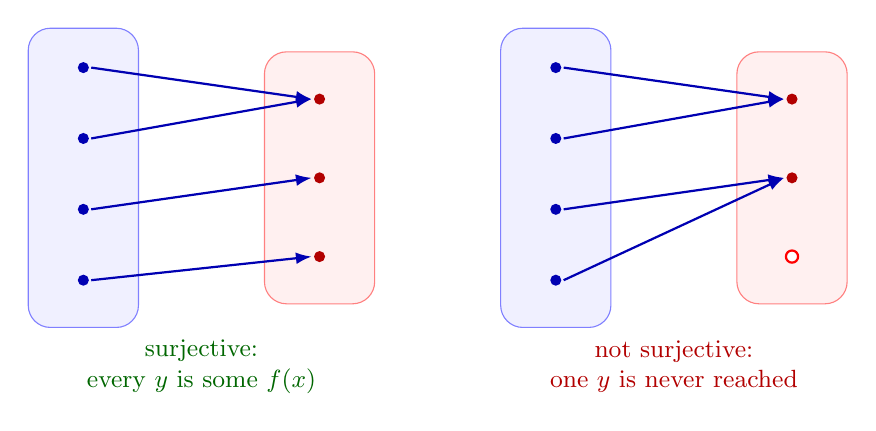
\begin{tikzpicture}[>={Latex[length=2mm]}, every node/.style={font=\small}]
	\begin{scope}
		\draw[rounded corners=8pt, fill=blue!6, draw=blue!50] (-0.7,-1.9) rectangle (0.7,1.9);
		\draw[rounded corners=8pt, fill=red!6, draw=red!50] (2.3,-1.6) rectangle (3.7,1.6);
		\foreach \y in {1.4,0.5,-0.4,-1.3} {\fill[blue!70!black] (0,\y) circle (2pt);}
		\foreach \y in {1.0,0,-1.0} {\fill[red!70!black] (3,\y) circle (2pt);}
		\draw[->, blue!70!black, thick] (0.1,1.4) -- (2.9,1.0);
		\draw[->, blue!70!black, thick] (0.1,0.5) -- (2.9,1.0);
		\draw[->, blue!70!black, thick] (0.1,-0.4) -- (2.9,0);
		\draw[->, blue!70!black, thick] (0.1,-1.3) -- (2.9,-1.0);
		\node[green!40!black, align=center] at (1.5,-2.4) {surjective:\\ every $y$ is some $f(x)$};
	\end{scope}
	\begin{scope}[xshift=6cm]
		\draw[rounded corners=8pt, fill=blue!6, draw=blue!50] (-0.7,-1.9) rectangle (0.7,1.9);
		\draw[rounded corners=8pt, fill=red!6, draw=red!50] (2.3,-1.6) rectangle (3.7,1.6);
		\foreach \y in {1.4,0.5,-0.4,-1.3} {\fill[blue!70!black] (0,\y) circle (2pt);}
		\foreach \y in {1.0,0} {\fill[red!70!black] (3,\y) circle (2pt);}
		\draw[red, thick, fill=white] (3,-1.0) circle (2.2pt);
		\draw[->, blue!70!black, thick] (0.1,1.4) -- (2.9,1.0);
		\draw[->, blue!70!black, thick] (0.1,0.5) -- (2.9,1.0);
		\draw[->, blue!70!black, thick] (0.1,-0.4) -- (2.9,0);
		\draw[->, blue!70!black, thick] (0.1,-1.3) -- (2.9,0);
		\node[red!70!black, align=center] at (1.5,-2.4) {not surjective:\\ one $y$ is never reached};
	\end{scope}
\end{tikzpicture}
\end{document}
